% !TEX root = ../zz-lecture.tex


\chapter{牛顿定律}

 牛顿运动定律是高中物理的基础,贯穿于高中物理的各个部分。
 在高中物理课程中,我们学习了牛顿运动定律的具体内容和基本应用。
 在未来的两次课中,我们将进一步研究牛顿第二定律(涉及分解加速度、加速度关联等问题)以及在非惯性系中如何使用牛顿第二定律。
 
 \stitle{牛顿第二定律}
 
 
 牛顿第二定律是矢量定律,因此可以分方向使用:
 \begin{equation}
 F_i = ma_i,
 \end{equation}
 其中$ i=1,2,3 $可以理解为力和加速度在给定直角坐标系中的$ x,y,z $分量。
在常规的高考问题中,一般是将外力沿加速度方向和垂直加速度方向进行正交分解,列出分量方程。
在一些复杂问题中,分解加速度列出分量方程可能会使问题更简化。

\begin{example}
	%%%%题干
	 如图所示,光滑的水平面上有甲、乙两个物体靠在一起,同时在水平力$ F_1 $和$ F_2 $的作用下运动.已知$ F_1>F_2 $,下列说法中正确的是(    )
	%%%%插图
		\marginpar{\centering 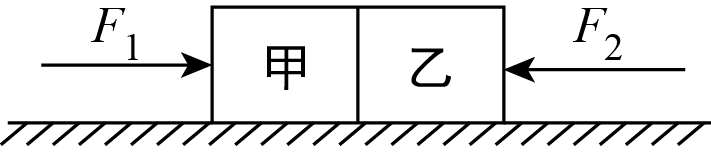
\includegraphics[width=0.8\marginparwidth]{image/newton-1}\figcaption{第\theexample 题 } }
		
		A.如果撤去$ F_1 $,甲的加速度一定会减小;
		
		B.如果撤去$ F_2 $,甲的加速度一定会减小;
		
		C.如果撤去$ F_2 $,乙的加速度一定会增大;
		
		D. 如果撤去$ F_1 $,乙对甲的作用力一定减小.
		
	
	\begin{taggedblock}{student}
		\vspace*{0cm}
	\end{taggedblock}
	
	
	%%%%答案
	\begin{taggedblock}{answer}
		答案:CD
	\end{taggedblock}
	
	
	%%%%解析
	\begin{taggedblock}{analysis}
		解析:
	\end{taggedblock}
\end{example}


\begin{example}
	%%%%题干
	如图所示,在光滑水平面上有一斜劈,其斜面倾角为$ \alpha $,一质量为$ m $的物体放在其斜面上,现用水平力$ F $推斜劈,恰使物体$ m $与斜劈间无相对滑动,则斜劈对物块$ m $的弹力大小为              .
	%%%%插图
		\marginpar{\centering 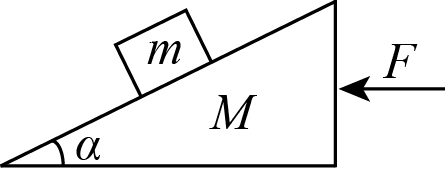
\includegraphics[width=0.8\marginparwidth]{image/newton-2.png}\figcaption{第\theexample 题 } }
	
	\begin{taggedblock}{student}
		\vspace*{1cm}
	\end{taggedblock}
	
	
	%%%%答案
	\begin{taggedblock}{answer}
		答案:$ mg\cos\alpha+\frac{m}{M+m}F\sin\alpha $
	\end{taggedblock}
	
	
	%%%%解析
	\begin{taggedblock}{analysis}
		解析:
	\end{taggedblock}
\end{example}



\begin{example}
	%%%%题干
	如图所示,在置于水平地面上的盛水容器中,用一端固定于容器底部的细线拉住一个空心的塑料球,使之静止地悬浮在深水中,此时容器底部对地面的压力记为$ N_1 $;某时刻拉紧球的细线突然断开后,球便在水中先加速后匀速地竖直上升,若球在此加速运动阶段和匀速运动阶段对应着容器底部对地面的压力分别记做$ N_2 $和$ N_3 $,则(    )
	
	A. 球加速上升时,$ N_1<N_2 $
	
	B. 球加速上升时,$ N_1>N_2 $
	
	C. 球匀速上升时,$ N_1<N_3 $
	
	D.  球匀速上升时,$ N_1>N_3 $
	
	
	%%%%插图
		\marginpar{\centering 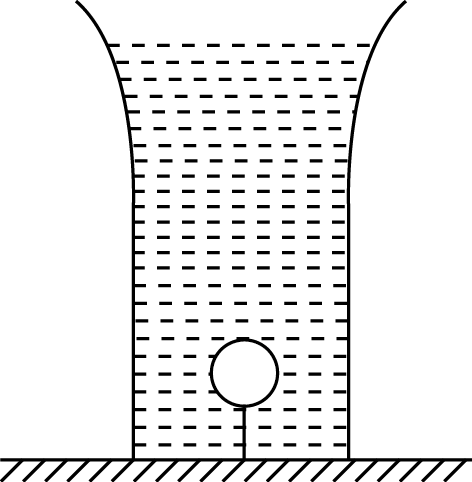
\includegraphics[width=0.8\marginparwidth]{image/newton-3.png}\figcaption{第\theexample 题 } }
	
	\begin{taggedblock}{student}
		\vspace*{0cm}
	\end{taggedblock}
	
	
	%%%%答案
	\begin{taggedblock}{answer}
		答案:B
	\end{taggedblock}
	
	
	%%%%解析
	\begin{taggedblock}{analysis}
		解析:球的加速上升和匀速上升可以认为与球等体积的水在加速下降和匀速下降.容器、水和球作为一个整体,塑料球静止和匀速运动时,系统处于平衡状态,地面对容器底部的支持力等于系统的重力.当球加速上升时,水加速下降,系统整体有向下的加速度,重力和支持力的合力提供加速度,所以重力大于支持力.故$ N_1=N_3>N_2 $故B正确,ACD错误.
	\end{taggedblock}
\end{example}


\begin{example}
	%%%%题干
	如图所示,质量为$ M $的劈块,其左右劈面的倾角分别为$\theta_1 = \deg{30},\theta_2 = \deg{45} $质量分别为$ m_1=\sqrt{3}~\si{kg}  $和$ m_2=2.0~\si{kg}  $的两物块,同时分别从左右劈面的顶端从静止开始下滑,劈块始终与水平面保持相对静止,各相互接触面之间的动摩擦因数均为$ \mu=0.20 $,求两物块下滑过程中($ m_1 $和$ m_2 $均未达到底端)劈块受到地面的摩擦力.取$ g = 10\si{m/s^2} $.
	%%%%插图
		\marginpar{\centering 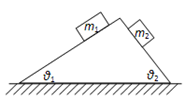
\includegraphics[width=0.8\marginparwidth]{image/newton-4.png}\figcaption{第\theexample 题 } }
	
	\begin{taggedblock}{student}
		\vspace*{2cm}
	\end{taggedblock}
	
	
	%%%%答案
	\begin{taggedblock}{answer}
		答案:$ f\simeq 2.1\si{N} $,方向向右;
	\end{taggedblock}
	
	
	%%%%解析
	\begin{taggedblock}{analysis}
		\begin{center}
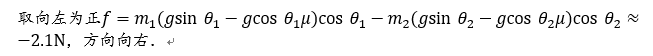
\includegraphics[width=0.9\linewidth]{image/newton-5}
\end{center}

	\end{taggedblock}
\end{example}


\begin{example}
	%%%%题干
	如图,$ m_1>m_2 $,滑轮质量和摩擦不计,则$ m_1 $和$ m_2 $匀加速运动的过程中,弹簧秤的读数是多少?
	%%%%插图
		\marginpar{\centering 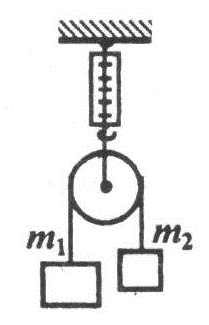
\includegraphics[width=0.8\marginparwidth]{image/newton-6.png}\figcaption{第\theexample 题 } }
	
	\begin{taggedblock}{student}
		\vspace*{2cm}
	\end{taggedblock}
	
	
	%%%%答案
	\begin{taggedblock}{answer}
		答案:$ F=(4m_1 m_2 g)/(m_1+m_2 ) $
	\end{taggedblock}
	
	
	%%%%解析
	\begin{taggedblock}{analysis}
			\begin{center}
				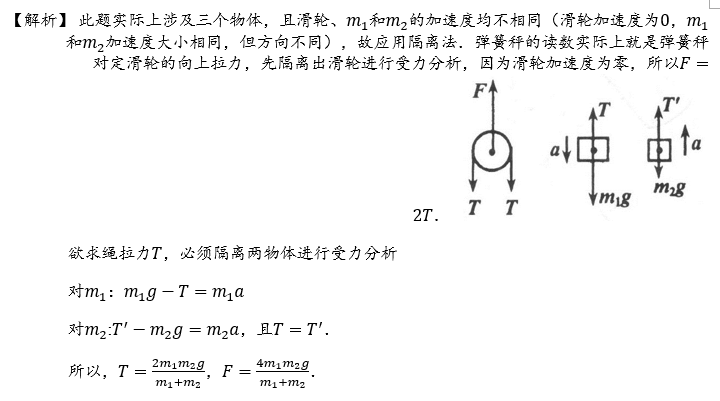
\includegraphics[width=0.9\linewidth]{image/newton-7}
			\end{center}
	\end{taggedblock}
\end{example}


\begin{example}
	%%%%题干
	如图所示,一根绳跨过装在天花板上的滑轮,一端接质量为M的物体,另一端吊一载人的梯子而平衡,人的质量为m,若滑轮与绳子的质量均不计,绳绝对柔软,不可伸长,为使滑轮对天花板的作用力为零,求人相对于梯子应按什么规律运动.
	%%%%插图
		\marginpar{\centering 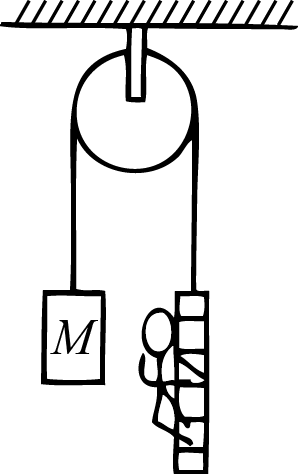
\includegraphics[width=0.6\marginparwidth]{image/newton-8.png}\figcaption{第\theexample 题 } }
	
	\begin{taggedblock}{student}
		\vspace*{2cm}
	\end{taggedblock}
	
	
	%%%%答案
	\begin{taggedblock}{answer}
		答案: 向下以相对速度$a_=2M/m g$做匀加速运动。
	\end{taggedblock}
	
	
	%%%%解析
	\begin{taggedblock}{analysis}
			\begin{center}
				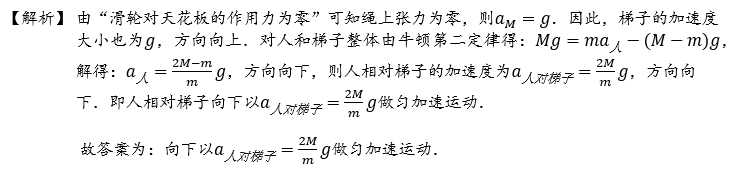
\includegraphics[width=0.9\linewidth]{image/newton-9}
			\end{center}
	\end{taggedblock}
\end{example}


\begin{example}
	%%%%题干
	如图所示,不计绳和滑轮质量,不计摩擦,A,B质量均为$ m $,剪断A上部的绳子,则B的加速度多大.
	%%%%插图
		\marginpar{\centering 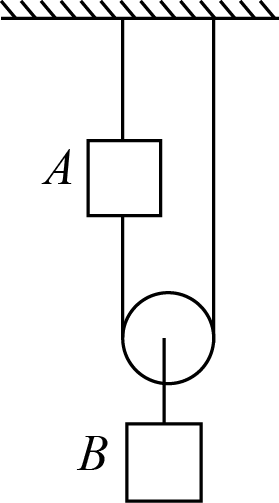
\includegraphics[width=0.6\marginparwidth]{image/newton-10.png}\figcaption{第\theexample 题 } }
	
	\begin{taggedblock}{student}
		\vspace*{2cm}
	\end{taggedblock}
	
	
	%%%%答案
	\begin{taggedblock}{answer}
		答案:$ a_B = \frac{3}{5}g $
	\end{taggedblock}
	
	
	%%%%解析
	\begin{taggedblock}{analysis}
		\begin{center}
			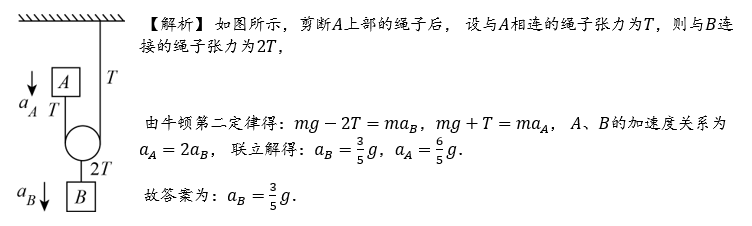
\includegraphics[width=0.9\linewidth]{image/newton-11}
		\end{center}
	\end{taggedblock}
\end{example}


\begin{example}
	%%%%题干
	如图所示,A、B、C三个物体的质量分别为$ m_1 $、$ m_2 $、$ m_3 $,所有接触面的摩擦均不计,绳、滑轮的质量也不计.求A、B、C运动时三个物体加速度的大小.
	%%%%插图
		\marginpar{\centering 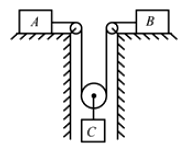
\includegraphics[width=0.8\marginparwidth]{image/newton-12.png}\figcaption{第\theexample 题 } }
	
	\begin{taggedblock}{student}
		\vspace*{2cm}
	\end{taggedblock}
	
	
	%%%%答案
	\begin{taggedblock}{answer}
		\begin{center}
			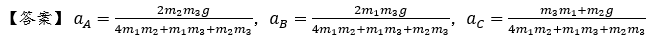
\includegraphics[width=0.9\linewidth]{image/newton-13}
		\end{center}
	\end{taggedblock}
	
	
	%%%%解析
	\begin{taggedblock}{analysis}
			\begin{center}
				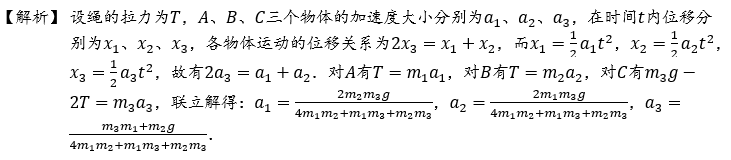
\includegraphics[width=0.9\linewidth]{image/newton-14}
			\end{center}
	\end{taggedblock}
\end{example}



\begin{example}
	%%%%题干
	如图所示,三个物体$ m_A = 1\si{kg},m_b = 2\si{kg},m_c = 3\si{kg} $,不计滑轮重力与摩擦,求C物体加速度.
	%%%%插图
		\marginpar{\centering 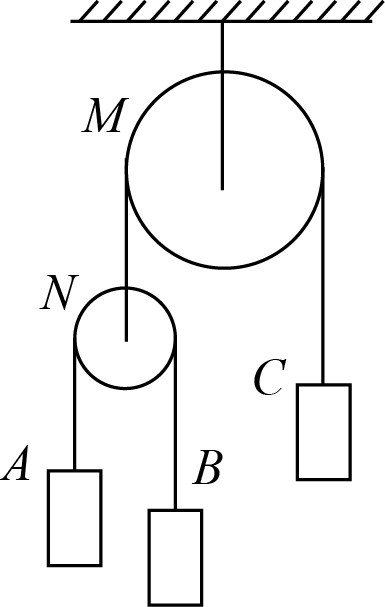
\includegraphics[width=0.7\marginparwidth]{image/newton-15.png}\figcaption{第\theexample 题 } }
	
	\begin{taggedblock}{student}
		\vspace*{2cm}
	\end{taggedblock}
	
	
	%%%%答案
	\begin{taggedblock}{answer}
		答案:$ a = \frac{g}{17} $
	\end{taggedblock}
	
	
	%%%%解析
	\begin{taggedblock}{analysis}
		解析:
	\end{taggedblock}
\end{example}


\begin{example}
	%%%%题干
	如图所示,一个质量为$ M $的小三角形物体$ A $放在倾角为$ \theta = \deg{30} $的固定斜面上,在此三角形上又放一质量为$ m $的物体B,A与B之间、A与斜面之间均光滑接触,设开始时A和B均静止.
	当A沿斜面下滑时,A对地面的加速度大小 $\underline{ \qquad\qquad }$             ,方向为 $\underline{ \qquad\qquad }$                 
	%%%%插图
		\marginpar{\centering 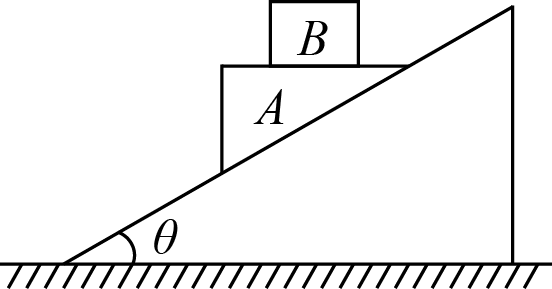
\includegraphics[width=0.8\marginparwidth]{image/newton-16.png}\figcaption{第\theexample 题 } }
	
	\begin{taggedblock}{student}
		\vspace*{2cm}
	\end{taggedblock}
	
	
	%%%%答案
	\begin{taggedblock}{answer}
		答案:$ \frac{2(M+m)g}{4M+m} $,沿斜面向下。
	\end{taggedblock}
	
	
	%%%%解析
	\begin{taggedblock}{analysis}
			\begin{center}
				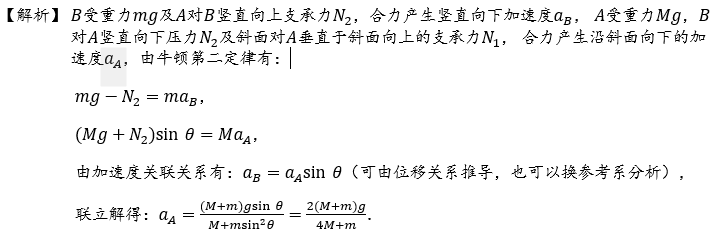
\includegraphics[width=0.9\linewidth]{image/newton-17}
			\end{center}
	\end{taggedblock}
\end{example}

\begin{example}
	%%%%题干
	如图所示,尖劈A的质量为$ m_A $,一面靠在光滑的竖直墙上,另一面与质量为$ m_B $的光滑棱柱B接触,B可沿光滑水平面滑动,求A、B的加速度$ a_A $和$ a_B $的大小及A对B的压力.
	%%%%插图
		\marginpar{\centering 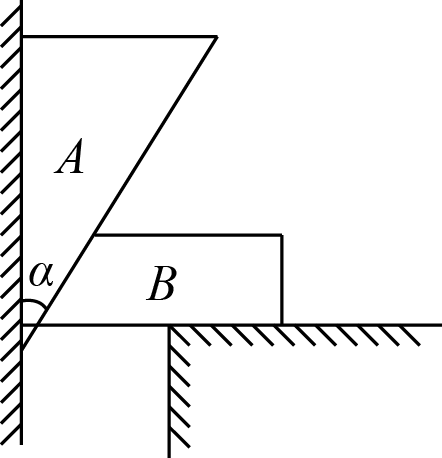
\includegraphics[width=0.8\marginparwidth]{image/newton-18.png}\figcaption{第\theexample 题 } }
	
	\begin{taggedblock}{student}
		\vspace*{2cm}
	\end{taggedblock}
	
	

	
	
	%%%%解析
	\begin{taggedblock}{analysis}
		\begin{center}
			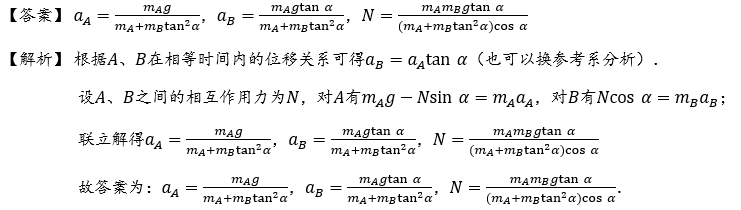
\includegraphics[width=\linewidth]{image/newton-19}
		\end{center}
	\end{taggedblock}
\end{example}


\begin{example}
	%%%%题干
	如图所示,斜面质量为$ M $,倾角为$ \alpha $;木杆只能沿竖直方向运动,质量为$ m $.一个水平力$ F $作用在斜面上,不记一切摩擦,求斜面的加速度.
	%%%%插图
	%	\marginpar{\centering 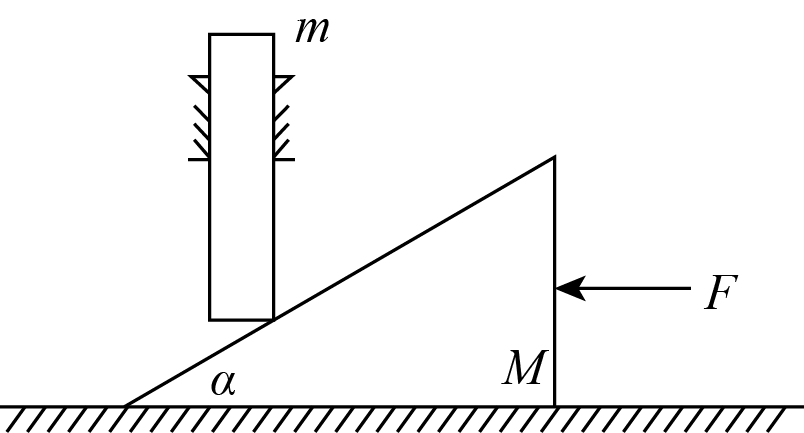
\includegraphics[width=0.8\marginparwidth]{image/newton-20.png}\figcaption{第\theexample 题 } }
	
	\begin{taggedblock}{student}
		\vspace*{2cm}
	\end{taggedblock}
	
	
	%%%%答案
	\begin{taggedblock}{answer}
		答案:$ a = \frac{F\cos\alpha-mg\sin\alpha}{M\cos\alpha+m\tan\alpha\sin\alpha} $
	\end{taggedblock}
	
	
	%%%%解析
	\begin{taggedblock}{analysis}
		解析:
	\end{taggedblock}
\end{example}


\begin{example}
	%%%%题干
	如图所示,一根长度为$ 3l $的轻杆上固定质量均为$ m $的两个重物,它们之间的距离以及它们分别到杆两端的距离相等.用两根竖直的绳子系在杆的两端,使杆水平放置且保持平衡状态.试求当右边绳子被剪断时刻两球的加速度.
	%%%%插图
		\marginpar{\centering 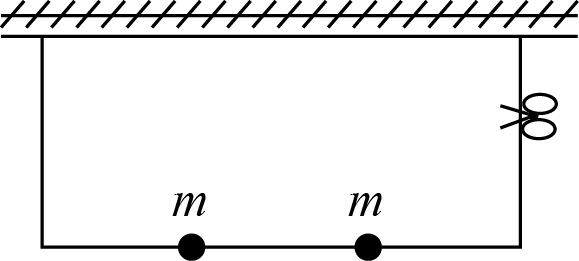
\includegraphics[width=0.8\marginparwidth]{image/newton-21.png}\figcaption{第\theexample 题 } }
	
	\begin{taggedblock}{student}
		\vspace*{2cm}
	\end{taggedblock}
	
	
	%%%%答案
	\begin{taggedblock}{answer}
		答案:$ a_1 = \frac{3}{5}g,a_2 = \frac{6}{5}g $
	\end{taggedblock}
	
	
	%%%%解析
	\begin{taggedblock}{analysis}
		\begin{center}
			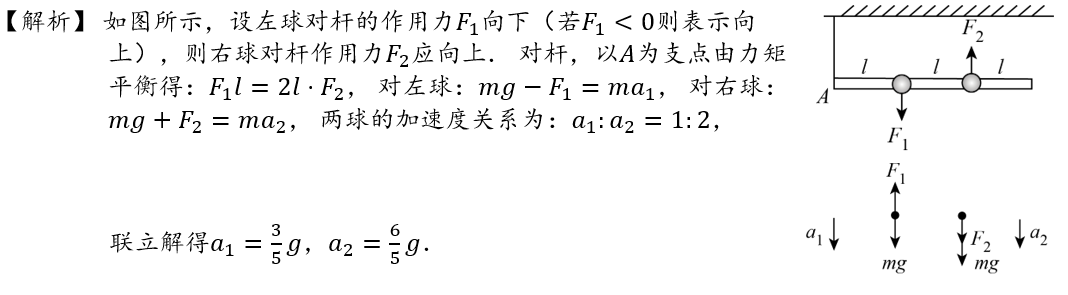
\includegraphics[width=\linewidth]{image/newton-22}
		\end{center}
	\end{taggedblock}
\end{example}


\begin{example}
	%%%%题干
	 如图所示,用两根长度均为l的完全相同的细线将一重物悬挂在水平的天花板下,细线与天花板的夹角为$ \theta $,整个系统静止,这时每根细线中的张力为$ T $.现在将一根细线剪断,在这一时刻另一根细线中的张力$ T' $为 $\underline{ \qquad\qquad }$  
	%%%%插图
		\marginpar{\centering 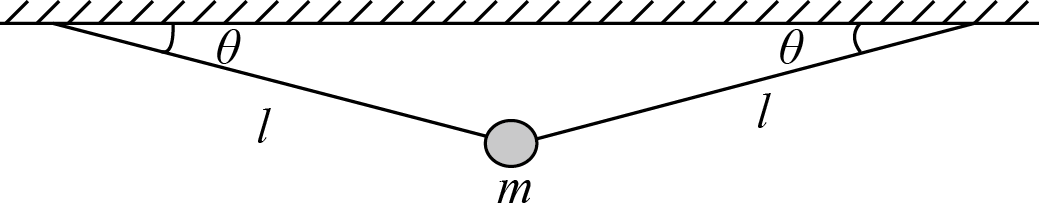
\includegraphics[width=\marginparwidth]{image/newton-23.png}\figcaption{第\theexample 题 } }
	
	\begin{taggedblock}{student}
		\vspace*{1cm}
	\end{taggedblock}
	
	
	%%%%答案
	\begin{taggedblock}{answer}
		答案:$ 2T\sin^2\theta $
	\end{taggedblock}
	
	
	%%%%解析
	\begin{taggedblock}{analysis}
		解析:	\begin{center}
			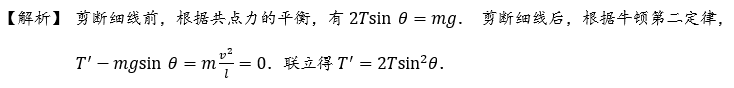
\includegraphics[width=\linewidth]{image/newton-24}
		\end{center}
	\end{taggedblock}
\end{example}



\begin{example}
	%%%%题干
	 如图所示,木棒AB质量均匀分布、质量大小为$ m $、长为$ 2l $,静止于光滑水平地面上.现给A端一微小扰动(近似认为扰动后速度仍为零),使AB沿逆时针方向倾倒,落地后不弹起.求AB翻倒到最终静止于水平地面的整个过程中,质心O点水平方向的位移.
	%%%%插图
	%	\marginpar{\centering \includegraphics[width=0.8\marginparwidth]{image/}\figcaption{第\theexample 题 } }
	
	\begin{taggedblock}{student}
		\vspace*{2cm}
	\end{taggedblock}
	
	
	%%%%答案
	\begin{taggedblock}{answer}
		答案:0
	\end{taggedblock}
	
	
	%%%%解析
	\begin{taggedblock}{analysis}
		解析:
	\end{taggedblock}
\end{example}
